% !TeX spellcheck = cs_CZ
%================ Kapitola 2: Unsere Familie ==============================================
\chapter{Lektion 4: Unsere Deutschstunde}\label{NJ:chap_N1_L4}

  Heute haben wir sechs Unterrichtsstunden. \textbf{Morgens beginnt der Unterricht um halb acht}. 
  Zuerst haben wir Mathematik, dann Geschichte. Fünfzehn Minuten vor zehn haben wir eine Pause.
  
  Punkt zwölf Uhr beginnt unsere Deutschstunde. Wir haben zweimal wöchentlich Deutsch, und zwar 
  montags und mittwochs. Mittwochs beginnt die Stunde aber erst um sechzehn Uhr dreißig und endet 
  um achtzehn Uhr. Da sind wir alle schon müde. Unser Lehrer ist jung, lustig und macht oft Witze. 
  Aber er ist auch streng. Wir müssen beim Unterricht immer gut aufpassen.
  
  Auch zu Hause sollen wir viel lernen, wir müssen Hausaufgaben machen, Vokabeln lernen und die 
  Grammatik wiederholen. Wir sollen auch deutsche Texte im Internet suchen. Es klappt nicht immer, 
  denn wir haben sehr wenig Zeit. Manchmal vergessen wir auch etwas. Aber heute ist es nicht so. 
  Wir sind alle auf unsere Deutschstunde gut vorbereitet. Zuerst korrigieren wir unsere Aufgaben. 
  Dann arbeiten wir mit dem Lehrbuch. Wir lesen und übersetzen Texte und üben die Grammatik. 
  Manche Übungen sind für uns noch ziemlich schwierig, wir verstehen oft nicht alles. Dann müssen 
  wir den Lehrer fragen. Er denkt bestimmt, wir sind dumm. Aber er erklärt uns alles noch einmal 
  und schreibt Beispiele an die Tafel. Wir machen auch Hörübungen mit dem Kassettenrecorder ohne 
  das Lehrbuch. Leider machen wir noch viele Fehler. Aber auch durch Fehler kann man viel lernen, 
  sagt unser Lehrer.
  
  Wir können schon ein wenig Deutsch sprechen. Der Lehrer stellt uns oft Fragen und wir antworten 
  auf Deutsch. Manchmal erzählen wir den Inhalt eines Textes, lösen Rätsel oder singen ein Lied. 
  Das Lernen macht uns Spaß. Glauben Sie es nicht? Doch, wir wollen ja bald gut Deutsch sprechen.
  
  \section*{Slovní zásoba}
    \begin{table}[ht!]   % L4_Wortschatz01.jpg L4_Wortschatz02.jpg
      \centering
      \begin{tabular}{llll}
        \hline
          e Stunde, -, n       & hodina {\scriptsize (trvání)}         & vor            
                                                    & před {\scriptsize (místně i časově)}        \\
          ohne (4.p.)          & bez(e)             & r Vorlesung      & přednáška                \\
          leider               & bohužel            & übersetzen       & přeložit                 \\
          e Übung, -, en       & cvičení   & s Beispiel, e(s), e       & příklad                  \\
          üben                 & cvičit    & vorbereitet (auf 4.p.)    & připravený (na)          \\
          lesen                & číst               & streng           & přísný, -ě               \\
          aufpassen            & dávat pozor        & schreiben        & psát                     \\
          heute                & dnes               & morgens          & ráno                     \\
          bis                  & do {\scriptsize (časově)}
                                                    & verstehen (4.p.) & rozumět (čemu),          \\
          singen               & zpívat             &                  & chápat                   \\
          zweimal              & dvakrát            & e Vokabel,-, n [wo-]  
                                                    & slovíčko {\scriptsize (ve slovníku)}        \\
          s Rätsel             & hádanka            & so               & tak                      \\
          dumm                 & hloupý, -ě         & ein wenig        & trochu                   \\
          e Uhr, -, 0          & hodina (čas)       & wöchentlich      & týdně                    \\
          e Uhr, -, en         & hodin(k)y          & sollen, ich soll 
                                                    & mít {\scriptsize (povinnost)}               \\
          r Fehler, s, -       & chyba              & s Lehrbuch, (e)s, ü-er  & učebnice          \\
          einmal               & jednou,            & r Lehrer, s, -   & učitel                   \\
                               & jedenkrát          & e Aufgabe, -, n  & úkol, úloha              \\
          s Buch, (e)s, ü-er   & kniha              & müde             & unavený, -ě              \\
          enden                & (s)končit          & bestimmt         & určitý, -ě               \\
          wenig                & málo               & montags        
                                                    & v pondělí {\scriptsize (obvykle)}           \\
          denken (an 4.p.)     & myslet (na)        & mittwochs      
                                                    & ve středu {\scriptsize (obvykle)}           \\
          denn                 & neboť              & lustig           & veselý, -e               \\
          etwas                & něco               & alle             & všichni                  \\
          mancher, manche      & některý, -á, -é    & r Witz, es, e    & vtip                     \\
          manches              & mnohý, -á, -é      & erzählen         & vyprávět                 \\
          e Tafel, -, n        & tabule             &  - (von/über 4.p.)  & vyprávět (o)          \\
          r Inhalt             & obsah              & lösen            & vyřešit                  \\
          schwierig            & obtížný, -ě        & erklären         & vysvětlit, -ovat         \\
          antworten {\scriptsize (auf 4.p.)} 
                               & odpovídat (na)     & r Unterricht, (e)s, 0  & vyučování          \\
          korrigieren          & opravovat          & ja               & vždyť                    \\
          s Lied               & piseň              & beginnen         & začít                    \\
          halb                 & poloviční          & vergessen (4.p.) & zapomenout (na)          \\
          stellen              & postavit, stavět   & wiederholen      & zopakovat                \\
          für                  & pro, za            & s Rätsel, s, -   & hádanka                  \\
        \hline
          r Inhalt, (e)s,      & obsah              & r Spaß, es, ä-e  & žert, zábava             \\
          e lösen              & (vy)řešit          & wollen, ich will & chtít                    \\
          ja {\scriptsize (uprostřed věty)} & vždyť, přece   & falsch  & špatný, -ě;              \\
          singen               & (za)zpívat         &                  & nesprávný, -ě            \\
          s Lied, (e)s, er     & píseň              & richtig          & správný, -ě              \\
        \hline 
      \end{tabular}
      \caption*{ }
    \end{table}
    \newpage
    \subsection*{Vazby}
      \begin{table}[ht!]   % L4_Redensart01.jpg
        \begin{tabular}{ll}
          \hline
          und zwar                            & a to                                             \\
          Da sind wir schon müde.             & To jsme už unaveni.                              \\
          Er macht oft Witze.                 & Často žertuje.                                   \\
          Es klappt nicht immer.              & Vždycky to nevyjde.                              \\
                                              & Vždycky se to nepodaří.                          \\
          Er stellt uns Fragen.               & Dává nám otázky.                                 \\
          Sagen Sie es auf Deutsch!           & Řekněte to německy!                              \\
          Das Lernen macht uns Spaß.          & Učení nás baví.                                  \\
          Wir wollen ja gut Deutsch sprechen. & Chceme přece                                     \\
                                              & Vždyť chceme mluvit dobře německy.               \\
          \hline
        \end{tabular}
        \caption*{ }
      \end{table}
      
    \begin{figure}[ht!]
      \centering
      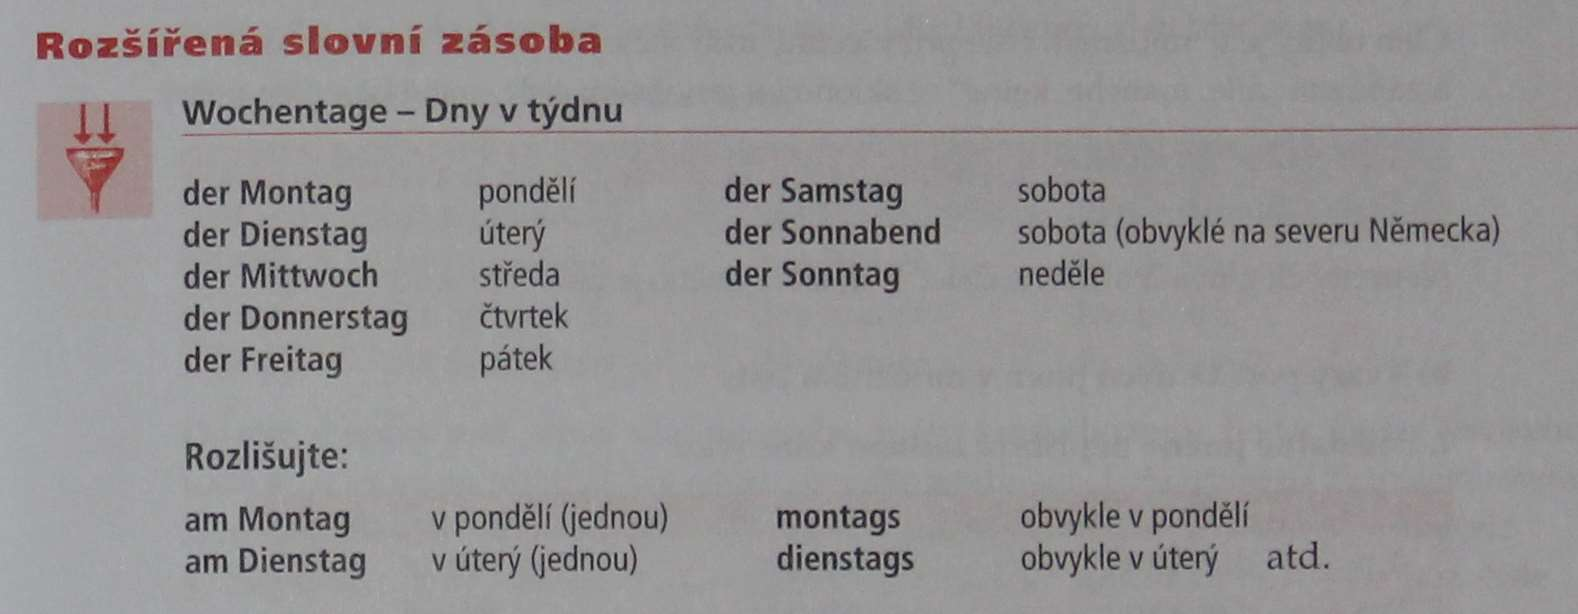
\includegraphics[width=1\linewidth]{L4_Wortschatz03.jpg}
      \caption*{ }
      \label{NJ:fig_L4_Wortschatz03}
    \end{figure}
    
    \subsection*{Skloňování podstatných jmen v množném čísle}
      \begin{itemize} % L4_Grammatik01.jpg
        \item \textbf{Skloňování určitého členu a některých zájmen v množném čísle:}
              \begin{table}[ht!]   % L4_Redensart01.jpg
                \hspace*{5em}
                \begin{tabular}{l|ll}
                  \hline
                  l.p. & die & meine, keine, alle, manche     \\
                  2.p. & der & meiner, keiner, aller, mancher \\
                  3.p. & den & meinen, keinen, allen, manchen \\
                  4.p. & die & meine, keine, alle, manche     \\
                  \hline
                \end{tabular}
                \caption*{ }
              \end{table}
              
              Člen určitý je v množném čísle pro všechny rody stejný. Všechna přivlastňovací 
              zájmena a zájmena „alle, manche, keine" se skloňují v množném čísle stejně jako člen 
              určitý.
              \begin{itemize}
                \addtolength{\itemindent}{5em}
                \item Haben Sie ein Kind?
                \item Haben Sie Kinder?
              \end{itemize}
              Neurčitý člen nemá množné číslo, podstatné jméno je pak bez členu.
        \item \textbf{Tvary podstatných jmen v množném čísle:}
          \begin{itemize}
            \item \textbf{Podstatné jméno nepřibírá žádnou koncovku}\newline
              \begin{table}[ht!]   % L4_Grammatik02.jpg
                \hspace*{4em}
                \begin{tabular}{l|lll}
                       & \textbf{der Vater}  & \textbf{die Mutter}  & \textbf{das Rätsel}  \\
                  \hline
                  1.p. & die Vater           & die Mütter           & die Rätsel           \\
                  2.p. & der Väter           & der Mütter           & der Rätsel           \\
                  3.p. & den Vätern          & den Müttern          & den Rätseln          \\
                  4.p. & die Väter           & die Mütter           & die Rätsel           \\
                  \hline
                \end{tabular}
                \caption*{ }
              \end{table}
        
              Bez koncovky jsou především podstatná jména mužského a středního rodu, která končí v 
              jednotném čísle na \textbf{-er}, \textbf{-el}, \textbf{-en} a zdrobněliny, které jsou 
              vždy středního rodu a tvoří se příponami \textbf{-chen} a \textbf{-lein}. Z 
              podstatných jmen ženského rodu jsou bez koncovky jen dvě - \emph{„die Mutter"} a 
              \emph{„die Tochter"}. Některá podstatná jména této skupiny přehlasují (tzn. mění 
              kmenovou samohlásku: \emph{a - ä}, \emph{u - ü}, \emph{o - ö}, \emph{au - äu}).
      
            \item \textbf{Podstatné jméno přibírá v množné čísle koncovku -e}\newline
              \begin{table}[ht!]   % L4_Grammatik02.jpg
                \hspace*{4em}
                \begin{tabular}{l|lll}
                       & \textbf{der Freund}   & \textbf{die Stadt}   & \textbf{das Jahr}    \\
                  \hline
                  1.p. & die Freunde           & die Städte           & die Jahre            \\
                  2.p. & der Freunde           & der Städte           & der Jahre            \\
                  3.p. & den Freunde\textbf{n} & den Städte\textbf{n} & den Jahre\textbf{n}  \\
                  4.p. & die Freunde           & die Städte           & die Jahre            \\
                  \hline
                \end{tabular}
                \caption*{ }
              \end{table}

              Tato skupina je zastoupena především u mužského rodu. V ženském rodě je zastoupena 
              pouze asi 40 podstatnými jmény, která přehlasují vždy, je-li v kmeni přehlasovatelná 
              samohláska. Podst. jména mužského a středního rodu přehlasují jen někdy.
              
            \item \textbf{Množné číslo má koncovku -er}\newline
            \item \textbf{Množné číslo má koncovku -(e)n}\newline
            \item \textbf{Množné číslo přebírá koncovku -s (pouze u některých cizích slov)}\newline
         \end{itemize}
      \end{itemize}
    
    \begin{figure}[ht!]
      \centering
      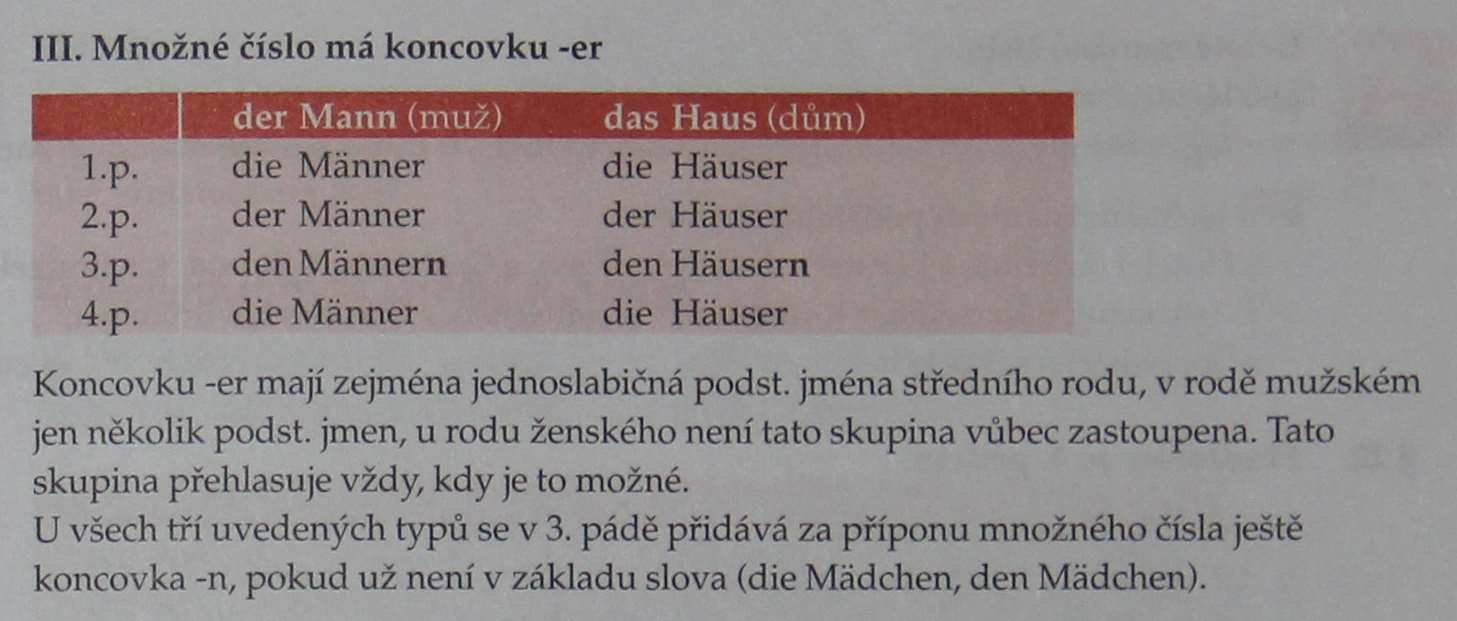
\includegraphics[width=1\linewidth]{L4_Grammatik03.jpg}
      \caption*{ }
      \label{NJ:fig_L4_Grammatik03}
    \end{figure}
    
    \begin{figure}[ht!]
      \centering
      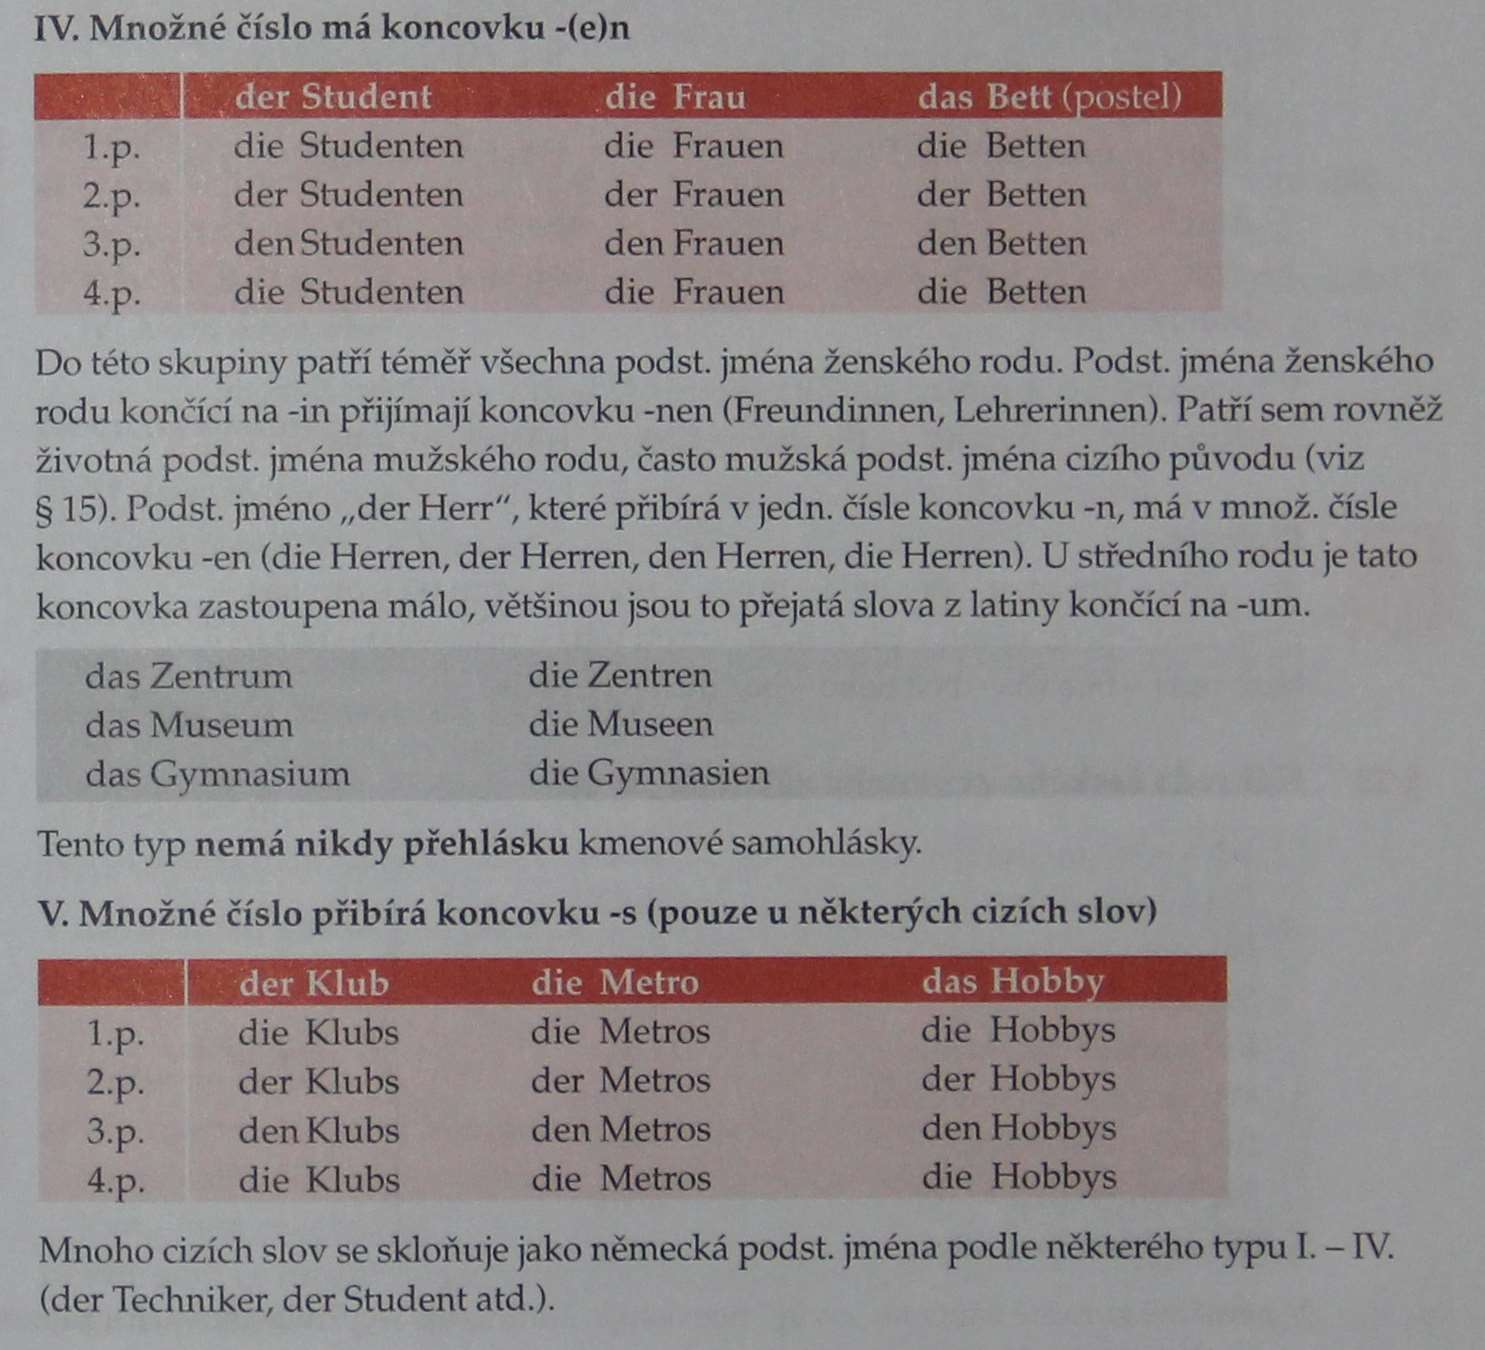
\includegraphics[width=1\linewidth]{L4_Grammatik04.jpg}
      \caption*{ }
      \label{NJ:fig_L4_Grammatik04}
    \end{figure}
    
    \begin{figure}[ht!]
      \centering
      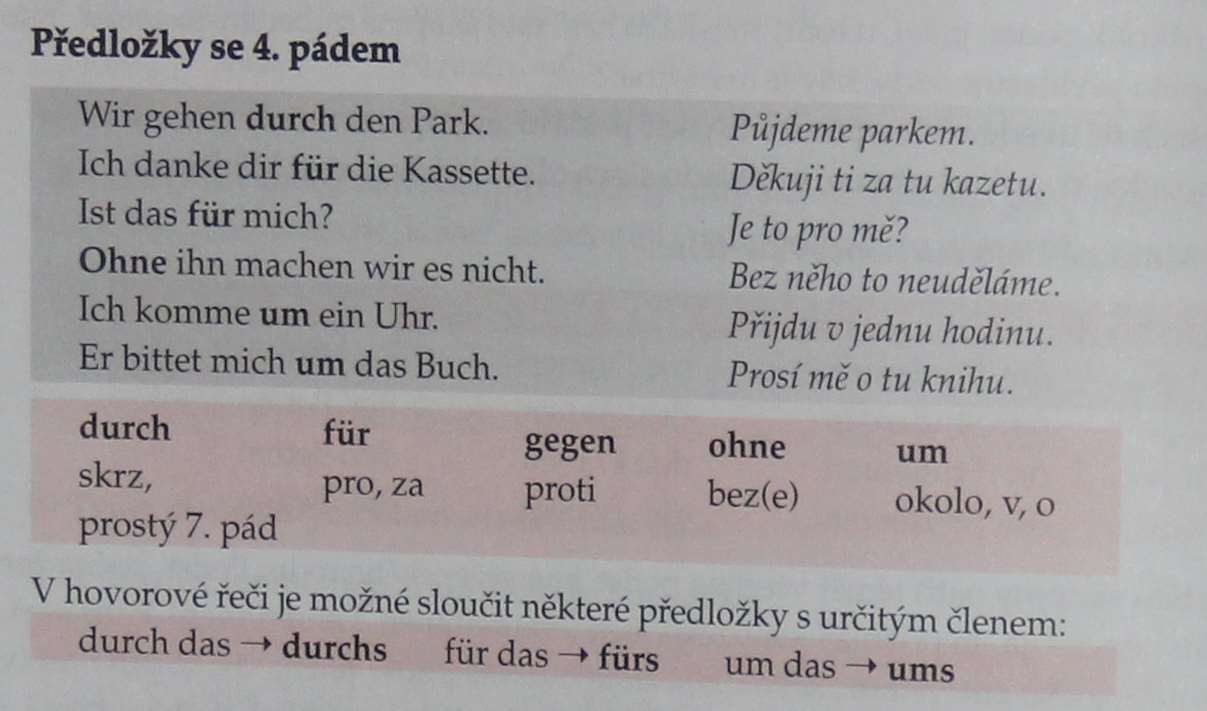
\includegraphics[width=1\linewidth]{L4_Grammatik05.jpg}
      \caption*{ }
      \label{NJ:fig_L4_Grammatik05}
    \end{figure}
    
    \begin{figure}[ht!]
      \centering
      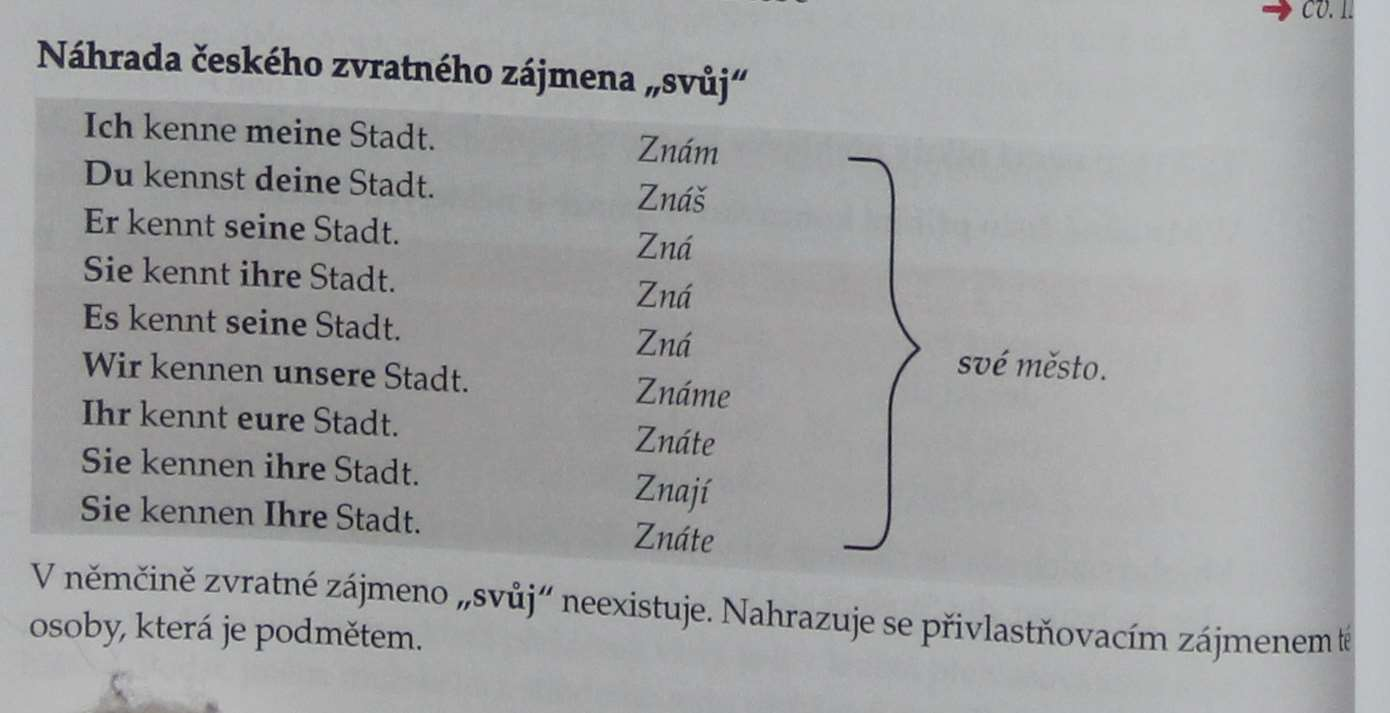
\includegraphics[width=1\linewidth]{L4_Grammatik06.jpg}
      \caption*{ }
      \label{NJ:fig_L4_Grammatik06}
    \end{figure}
    
    \begin{figure}[ht!]
      \centering
      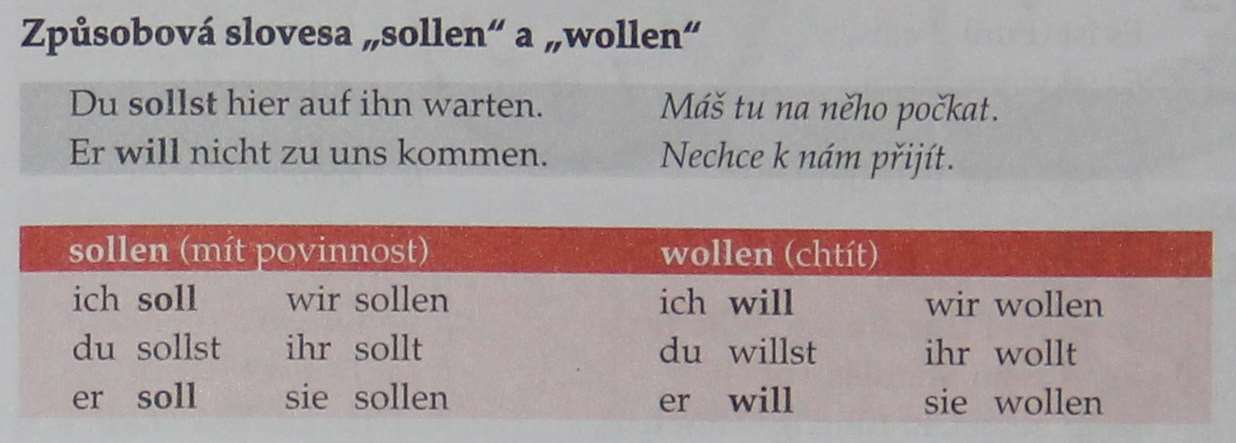
\includegraphics[width=1\linewidth]{L4_Grammatik07.jpg}
      \caption*{ }
      \label{NJ:fig_L4_Grammatik07}
    \end{figure}
    
    \begin{figure}[ht!]
      \centering
      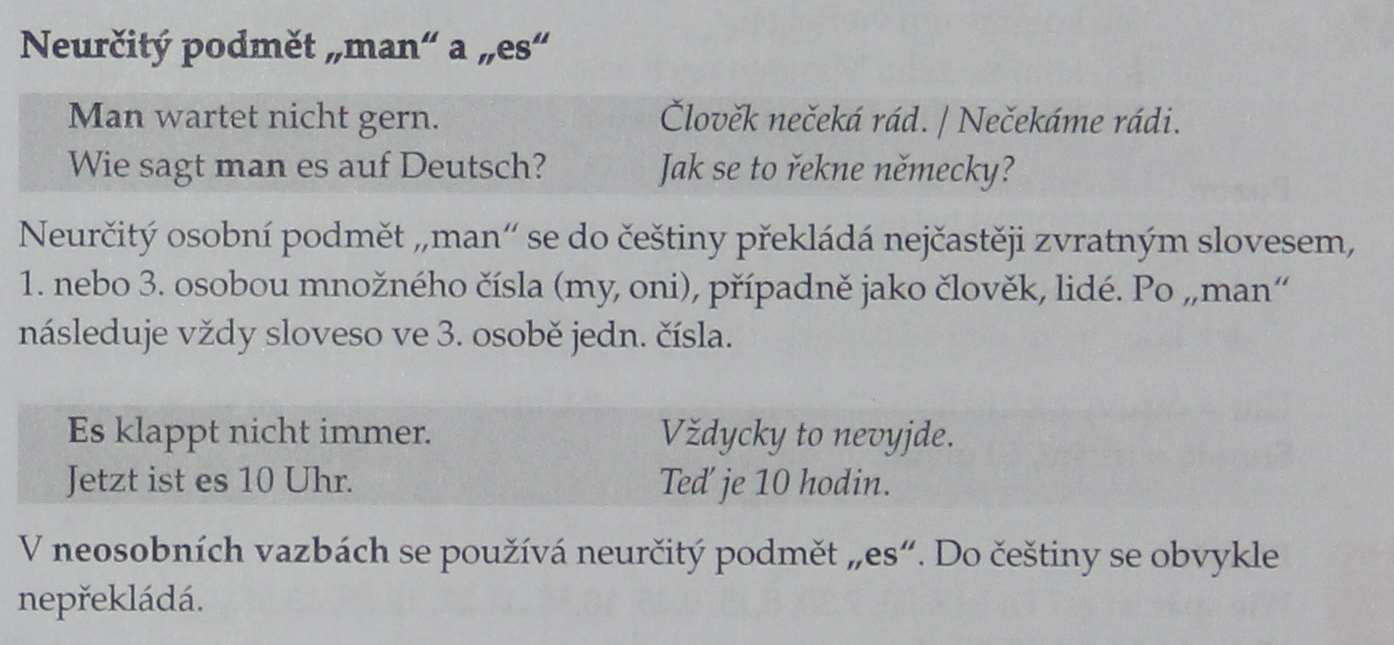
\includegraphics[width=1\linewidth]{L4_Grammatik08.jpg}
      \caption*{ }
      \label{NJ:fig_L4_Grammatik08}
    \end{figure}